\documentclass[12pt, a4paper]{report}

\usepackage[margin=20mm]{geometry}
\usepackage{calc}
\usepackage[default]{sourcesanspro}
\usepackage{tikz}
\usepackage{etoolbox}
\usepackage{hyperref}
\usepackage[none]{hyphenat}
\usepackage{amssymb}
\usepackage{amsmath}
\usepackage{longtable}
\usepackage{booktabs}
\usepackage{fancyhdr}
\usepackage[toc]{glossaries}
\usepackage[lofdepth,lotdepth]{subfig}
\usepackage{graphicx}

\usepackage{float}
\floatplacement{figure}{h}

\usepackage{xcolor}
\definecolor{white}{HTML}{FFFFFF}
\definecolor{black}{HTML}{000000}
\definecolor{green}{HTML}{198701}
\definecolor{orange}{HTML}{FF6138}
\definecolor{red}{HTML}{ba0900}
\definecolor{blue}{HTML}{0B75CB}
\definecolor{yellow}{HTML}{EFC82B}
\definecolor{purple}{HTML}{49075E}
\definecolor{webpage}{HTML}{a18613}
\definecolor{webpagesecond}{HTML}{1975FF}
\colorlet{primary}{webpage}
\newcommand{\primary}[0]{\color{primary}}
\newcommand{\black}[0]{\color{black}}

\usetikzlibrary{shapes.geometric, arrows, fit}
\tikzstyle{process} = [rectangle, minimum width=3cm, minimum height=1cm, text centered, draw=black, fill=orange!30]
\tikzstyle{page} = [rectangle, minimum width=3cm, minimum height=1cm, text centered, draw=black, fill=primary!30, rounded corners=4pt]
\tikzstyle{menu} = [rectangle, minimum width=3cm, minimum height=1cm, text centered, draw=black, fill=webpagesecond!30, rounded corners=4pt]
\tikzstyle{group} = [rectangle, minimum width=3cm, minimum height=1cm, text centered, draw=black, thick]
\tikzstyle{arrow} = [thick,<->,>=stealth]

\usepackage[colorinlistoftodos,color=primary]{todonotes}

\usepackage{framed}
\usepackage[framemethod=TikZ]{mdframed}
\newcounter{note}\setcounter{note}{0}
\renewcommand{\thenote}{\arabic{note}}
\newenvironment{note}[1]{
	\begin{minipage}{\linewidth}
		\vspace{1em}
		\stepcounter{note}
		\ifstrempty{#1}{
			\mdfsetup{
				frametitle={
					\tikz[baseline=(current bounding box.east),outer sep=0pt]
					\node[anchor=east,rectangle,fill=primary!20]
					{\strut Note~\thenote};
				}
			}
		}{
			\mdfsetup{
				frametitle={
					\tikz[baseline=(current bounding box.east),outer sep=0pt]
					\node[anchor=east,rectangle,fill=primary!80,rounded corners=4pt]
					{\strut~#1};
				}
			}
		}
		\mdfsetup{roundcorner=10pt,innertopmargin=0pt,linecolor=primary!80,linewidth=2pt,topline=true,frametitleaboveskip=\dimexpr-\ht\strutbox\relax}
		\begin{mdframed}[]\relax
		}{
	\end{mdframed}\end{minipage}
}
\renewenvironment{leftbar}[1][\hsize]
{
    \def\FrameCommand
    {
        {\color{primary}\vrule width 2pt}
        \hspace{0pt}%must no space
        \fboxsep=\FrameSep\colorbox{primary!10}
    }
    \MakeFramed{\hsize#1\advance\hsize-\width\FrameRestore}
}
{\endMakeFramed}

\newcommand{\persona}[5]{
	\begin{note}{#1}
		\begin{description}
			\item[Age:] #2
			\item[Gender:] #3
			\item[Goals:]
			\item[]#4
			\item[Pain Points:]
			\item[]#5
		\end{description}	
	\end{note}
}

% set the title format
\usepackage[explicit]{titlesec}
% \usepackage{xhfill}
\newcommand{\vrulefill}[1]{\leavevmode\leaders\hrule height#1\hfill\kern0pt}
\newcommand{\firstletter}[1]{\primary#1\black}
\newcommand{\ruleafter}[1]{#1~\xrfill[.7ex]{1pt}}
\titleformat{\section}{\bfseries\primary\Large}{\thesection}{0.75em}{#1\quad\vrulefill{0.12em}}
\titlespacing*{\section}{0em}{3em}{0em}
\titleformat{\subsection}{\bfseries\primary\large}{\thesubsection}{0.75em}{#1}
\titlespacing*{\subsection}{0em}{1em}{0em}
\def\myfirstletter#1{\primary#1\black}
\DeclareRobustCommand{\FirstPrimaryLetter}[1]{\myfirstletter #1}
\titleformat{\subsubsection}[hang]{\bfseries\large}{}{0em}{\quad\FirstPrimaryLetter#1}
\titlespacing*{\subsubsection}{0em}{1em}{0em}
\setcounter{secnumdepth}{3}
\renewcommand\contentsname{Table of Contents}
\setlength\parindent{0pt}

% set the item spacing
\usepackage{enumitem}
\setlist{nosep}

\fancyfoot{}
\fancyhead{}
\fancyhead[L]{\leftmark}
\fancyhead[R]{\rightmark}
%\fancyhead[C]{Design Report}
\fancyfoot[R]{Page\ \thepage}
\fancyfoot[L]{DECO1400}
\fancyfoot[C]{Daniel Fitzmaurice (\primary 43961229\black)}
\renewcommand{\headrulewidth}{0.15em}
\renewcommand{\footrulewidth}{0.15em}
\renewcommand{\headrule}{\hbox to\headwidth{\primary\leaders\hrule height\headrulewidth\hfill}}
\renewcommand{\footrule}{\hbox to\headwidth{\primary\leaders\hrule height\footrulewidth\hfill}}

\makeglossaries
\newacronym{api}{API}{Application Programming Interface}
\newacronym{html}{HTML}{HyperText Markup Language}
\newacronym{os}{OS}{Operating System}
\newacronym{ux}{UX}{User Experience}
\newglossaryentry{javascript}{
	name={JavaScript},
	description={Browser scripting language used to provide interactive features}
}
\newglossaryentry{react}{
	name={React},
	description={JavaScript framework which utilizes the virtual DOM and component based tree structure to improve application performance and reduce code duplication}
}
\newglossaryentry{typescript}{
	name={TypeScript},
	description={Adds static type checking to JavaScript}
}
\newglossaryentry{smarthome}{
	name={SmartHome},
	description={An environment in which a series of different devices communicate and interact together to provide an end user with a more automated housing experience}
}
\newglossaryentry{git}{
	name={Git},
	description={A popular version control system for tracking a change history of code and providing easily collaboration between developers. Git is commonly used with an online public repository such as GitHub or GitLab}
}
\newglossaryentry{byte}{
	name={Byte},
	description={Most common type of datatype in an electronic system, also sometimes considered the smallest}
}
\newglossaryentry{hex}{
	name={Hex},
	description={A number system of base 16, commonly used in computer systems because a group of two hex numbers makes up a \gls{byte}}
}
\newglossaryentry{opensource}{
	name={Open Source},
	description={Associated with a project where all code and content required for the project is accessible publicly and can be contributed to with respect to any associated licensing}
}

\begin{document}
	% !TeX spellcheck = en_US
% !TeX root = main.tex
\begin{titlepage}
\begin{center}

\begin{minipage}{\textwidth}
	\begin{center}
		\begin{minipage}{\widthof{\Huge Daniel Fitzmaurice}}
			\Huge
			Daniel Fitzmaurice\\
			\vspace{1em}
			\hfill(\primary 43961229\black )\\
		\end{minipage}
	\end{center}
	\vspace{10em}
\end{minipage}
\begin{minipage}{\textwidth}\begin{center}
		
\includegraphics{logo}\\\vspace{0em}
		\huge University of Queensland\\
		\LARGE\color{primary}\textbf{DECO1400}\color{black}\ -- Introduction to Web Design\\\vspace{2em}
		Design Report
\end{center}\end{minipage}


\begin{tikzpicture}[remember picture,overlay,shorten >= -10pt]
	\coordinate (aux1) at ([yshift=-15pt]current page.north east);
	\coordinate (aux2) at ([yshift=-410pt]current page.north east);
	\coordinate (aux3) at ([yshift=-4.5cm]current page.north east);
	\coordinate (aux4) at ([yshift=-150pt,xshift=-20pt]current page.north east);
	\coordinate (aux5) at ([yshift=-8cm,xshift=-40pt]current page.north east);
	\coordinate (aux6) at ([yshift=-10cm,xshift=-25pt]current page.north east);
	\coordinate (aux7) at ([yshift=-13cm,xshift=-50pt]current page.north east);
	
	\coordinate (bottom1) at ([xshift=10pt,yshift=30pt]current page.south west);
	\coordinate (bottom2) at ([xshift=40pt]current page.south west);
	\coordinate (bottom3) at ([xshift=120pt]current page.south west);
	\coordinate (bottom4) at ([xshift=220pt,yshift=30pt]current page.south west);
	\coordinate (bottom5) at ([xshift=180pt]current page.south west);
	
	\begin{scope}[primary,line width=12pt]
		\draw[opacity=0.6] (aux1) circle (3cm);
		\draw[opacity=0.4] (aux2) circle (2cm);
		\draw[opacity=0.7] (aux3) circle (3.5cm);
		\draw[opacity=0.5] (aux4) circle (2cm);
	\end{scope}
	\begin{scope}[primary!70,line width=8pt]
		\draw[opacity=0.7] (aux5) circle (2.5cm);
		\draw[opacity=1] (aux6) circle (1.5cm);
		\draw[opacity=0.8] (aux7) circle (2cm);
	\end{scope}
	
	\begin{scope}[primary,line width=8pt]
		\draw[opacity=0.5] (bottom1) circle (2.5cm);
		\draw[opacity=0.6] (bottom2) circle (2cm);
		\draw[opacity=0.3] (bottom3) circle (3.5cm);	
		\draw[opacity=0.7] (bottom4) circle (2.5cm);
		\draw[opacity=0.6] (bottom5) circle (2cm);
	\end{scope}


\end{tikzpicture}

\end{center}
\end{titlepage}
	\newpage
	\pagenumbering{roman}
	\tableofcontents
	\listoffigures
	%\listoftables
	\printglossary
	\newpage
	
	\pagestyle{fancy}
	\pagenumbering{arabic}
	
	\chapter{Design and Details}
	% !TeX spellcheck = en_US
% !TeX root = main.tex

\section{Introduction}
% Who and what is this design report for?
% What can we expect from the follow pages?

\subsection{Introduce Yourself}
% Briefly describe yourself
% What's your background?
% What's your skills, interests, degree, etc
% What's your learning strategy (as defined in the Week 1 practical) at the start of the course
	% !TeX spellcheck = en_US
% !TeX root = main.tex

\section{Getting to Know Stakeholders}
\subsection{Target Audience}
% Who is the specific target audience in relation to the brief?
% Include a few personas that represent different, archetypal users
% What are some common traits you've identified from your personas?
% What implications does this audience have for the design?
It is always essential to pick a target audience for a project before beginning, this will help to identify relevant content and ideas that should or should not be used. For this project the target audience is centred around people just beginning to learn about code or beginning to enter a professional environment where their code or actions will be marked and versioned. These sorts of people at typically around 18 to 22 years old and have some basic experience with computers and know how to work their way around the system. However they are still incredibly knew to the environment and if content is not broken down in an understandable way then they can be easily confused and lose interest.

\subsubsection{Goals}
With the target audience specified it can now be import to outline goals that should be followed to ensure the target audience is engaged.
\todo[inline]{Get all the references}
\begin{description}
	\item[Consumable Chunks:] The target audience require information to be broken down into consumable chunks in which they can learn, reflect, and then use before moving on to the next chunk.
	\item[Direct Content Flow:] Content chunks should also logically flow from one section to the next without large gaps in presentation. Not following this goal will ultimately result in the consumer losing track and becoming disinterested.
	\item[Simplistic Graphics:] Following design patterns released by large web driven companies, such as Google and Facebook, content should be shown in a way that is not overcrowded and can be confusing. If graphics are used to illustrate a point they should be vector based to help provide a more defining and clean look.
	\item[Defined Website Theme:] In order to engage the users and not make them lose interest, the website must have a clear and engaging theme that is applied site wide. This will help to reduce confusion about different sections of the site.
	\item[Clean and Polished:] The site as a whole should be clean and usable site. This means performance should remain consistent and have an expected behaviour across the entire site. As well all graphics should be presented in a high quality and consistent manor, this can be achieved using vector graphics and rendering on the client side. Finally the site should function across all modern browsers and devices, as well as having accessibility support.
\end{description}


\subsection{Chosen Educational Content}
% What is your chosen educational content?
% Why is this educational content an interesting choice for the target audience?
For this website, the goal is to be a resource for people wanting to learn about git the version source control system. Git allows people to track and mark changes they are making to code as well as easily allowing other people to integrate and edit the code together. Git fits well into the target audience because it is becoming more and more essential programming jobs and is becoming assumed knowledge for every programmer. Therefore people just starting in industry might not have knowledge about this tool and therefore need to upskill quickly and efficiently.

\subsection{Chosen Story}
% What is your chosen story and genre?
% Why is this story an interesting choice for the website's visuals and theme in relation to the target audience?
\todo[inline]{Find a story}
	% !TeX spellcheck = en_US
% !TeX root = main.tex

\section{Navigation and Organisation}
\subsection{Card Sorting}
% Reflect on the success of the Card Sorting design activity you did in Week 4
% Include the testing plan you developed for the activity
% Include photos you took of the activity running
% What feedback did you get and how did it inform your early content organisation decisions?
% Which organisation systems will you use in your website and why?

\subsubsection{The Plan}
To begin there were three main areas of content were identified: Git Reference Summary, Main storyline/tutorial, Interactive Quiz. These areas were then assigned a rank and associated keywords:
\begin{itemize}
	\item\textbf{Git Reference Summary}
	\begin{itemize}
		\item Shows all the commands and a basic overview of what they do
		\item This will be visited most by people coming back because they forgot something or wanted to know more outside of the main storyline
		\item \textbf{Rank:} 2
		\item \textbf{Keywords:} Advanced, Reflection, Quick
	\end{itemize}
	\item\textbf{Main storyline/tutorial}
	\begin{itemize}
		\item This will be most frequently visited by new comers and people just visiting the site
		\item \textbf{Rank:} 1
		\item \textbf{Keywords:} Beginner, Interesting, Interactive
	\end{itemize}
	\item\textbf{Interactive Quiz}
	\begin{itemize}
		\item Some of this will also be embedded inside the storyline
		\item People wanting a challenge and to learn more
		\item \textbf{Rank:} 3
		\item \textbf{Keywords:} Self Learning, Interactive, All Levels
	\end{itemize}	
\end{itemize}

For this survey I chose to go with an Open Card Sort because I wanted to observe how they thought about grouping and what is easier or more important to sort before arriving at a final decision. After the users had finished with sorting the cards, a couple of follow up questions/discussions would be had around why they named the groups they did.

\subsubsection{Execution}
In order to execute the card sorting, Trello was used for the physical moving of cards around. This decision was made because it best allows people to move the cards around like they would physically, while still providing them with the easy of changing the names of the groups.

\subsubsection{Results}
\begin{note}{Person 1}
	\begin{figure}[H]
		\centering
		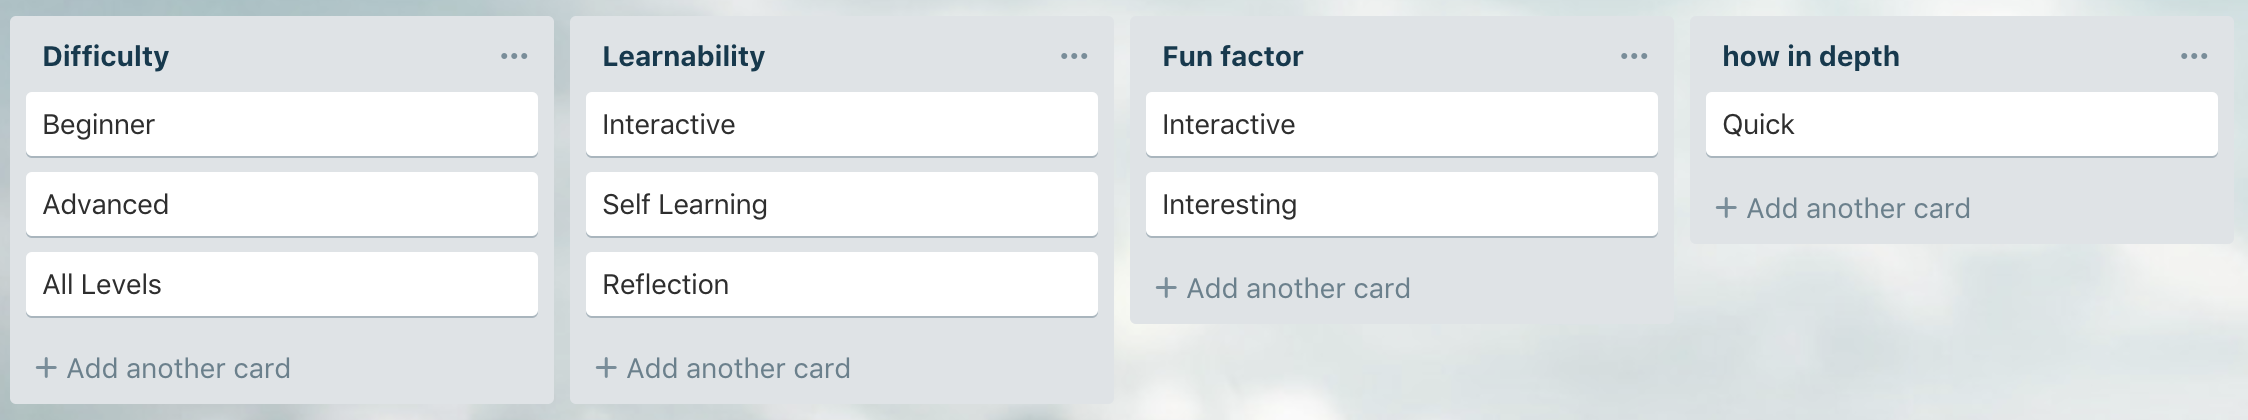
\includegraphics[width=\linewidth]{card1}	
		\caption{Person 1's Card Sorting Result}
	\end{figure}

	How did you group the tags?
	\begin{leftbar}
		Beginner and advanced are varying difficulties, I don't know if that is something I can choose. All levels are associated, can I filter by difficulty level on the side.\\\\
		Grouped them because the concepts are the same, but on the site I wouldn't expect beginner and advance to be together.
	\end{leftbar}

	How did you name the groups?
	\begin{leftbar}
		\begin{itemize}
			\item Difficulty
			\begin{itemize}
				\item When you play a video game you pick your difficulty level
			\end{itemize}
			\item Learnability
			\begin{itemize}
				\item Self learning, learnability makes sense
				\item Interactive is key to learning
				\item Reflection is key to learning, gauge how successful you were
			\end{itemize}
			\item Fun Factor
			\begin{itemize}
				\item Interactive website's are fun, reading a static page can be quite passive and boring
				\item It's interesting because I am curious and it feels more tactile
			\end{itemize}
			\item How in Depth (\textit{mean not very in depth})	
			\begin{itemize}
				\item I would go through the site really quickly
				\item So the level of detail in the website is probably really shallow
			\end{itemize}
		\end{itemize}
	\end{leftbar}
\end{note}

\begin{note}{Person 2}
	\begin{figure}[H]
		\centering
		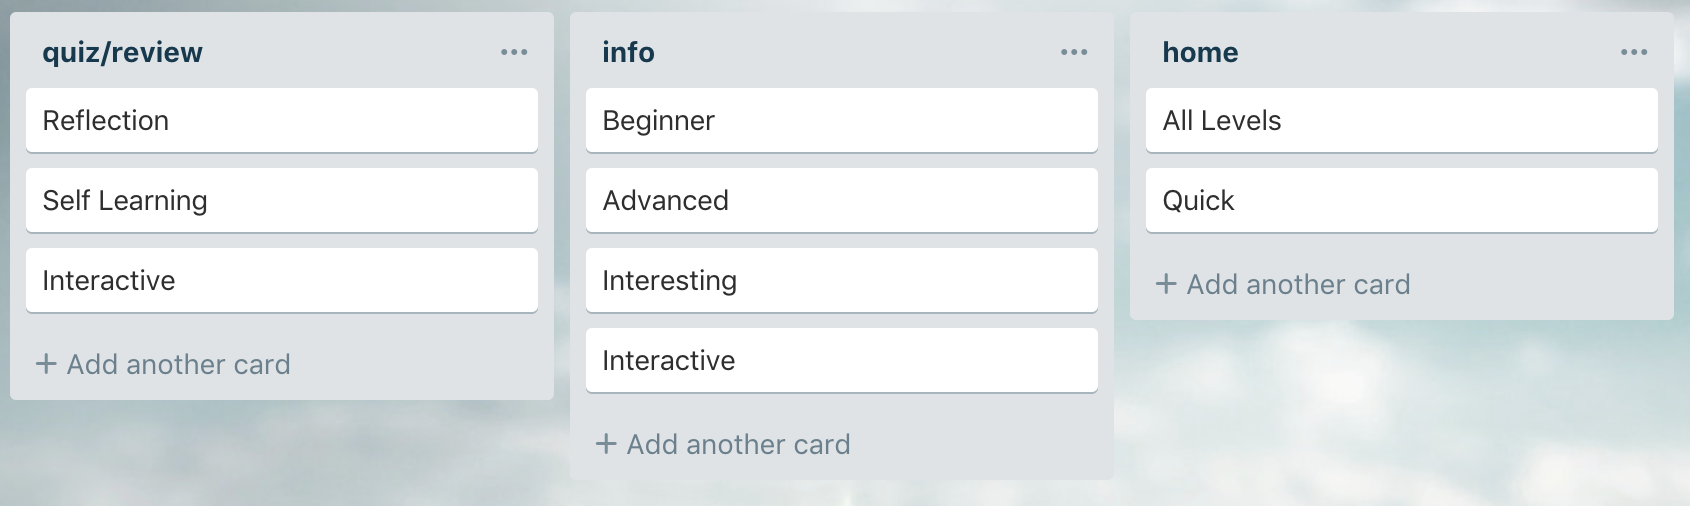
\includegraphics[width=\linewidth]{card2}	
		\caption{Person 2's Card Sorting Result}
	\end{figure}

	How did you group the tags?
	\begin{leftbar}
		Beginner and advanced are linked and interesting is cool\\\\
		All Levels and Quick are navigation type\\\\
		Reflection/SL/Interactive seem like quizzing	
	\end{leftbar}
	
	How did you name the groups?
	\begin{leftbar}
		\begin{itemize}
			\item Quiz/Review
			\begin{itemize}
				\item Reflection/SL is like looking back at what you learnt
				\item Looking back
			\end{itemize}
			\item Info
			\begin{itemize}
				\item Looking at Beginner and Advanced and interactive is like the middle of where you go
				\item Middle man of the navigation
			\end{itemize}
			\item Home
			\begin{itemize}
				\item They seem like navigation and be able to go through the site
			\end{itemize}
		\end{itemize}
	\end{leftbar}
\end{note}



\subsection{Navigation Systems}
% What were the key things you learned from your Navigation Systems group discussion?
% Write a brief response of your own to the guiding questions for this group discussion
% Which navigation systems will you use in your website and why?
A lot of the shown ``correct'' styles of navigation systems followed a similar style and placement. A lot of incorrect styles were outside the norm of having common elements. These elements are:
\begin{itemize}
	\item A main banner which include a general logo and quick navigation links underneath
	\item Most of the examples also used an inner page navigation panel on the left for filtering content on the current page	
\end{itemize}
Reflecting on the themes and the presentation styles used across websites that are considered good design, a similar layout will be used for this website. However slight modifications will be made to suit a scrolling storyline layout. To increase screen size and make the website appear more story like, the main logo will be reduced to be inline with the primary navigation menu. A side navigation menu will be created but it will be semi-hidden for a majority of the website and only showing itself when the mouse interacts with the shown tip.


\subsection{Site Map}
% Draw a site map that visualises the navigation flow of your website
% Include any internal (between pages) and external links
% Storyboard how one of your personas will navigate your website

\subsection{Visual Organisation}
% What were the key things you learned from you Visual Organisation group discussion?
% Write a brief response of your own to the guiding questions for this group discussion

\subsection{Interactivity and Functionality}
% Draw wireframes for each type of page in your website (i.e. if you have 5 pages that function very similarly, you only need to draw 1 wireframe)
% These can be derived from the same mockups you produced for Paper Prototyping
% Add annotations to describe:
% - how each interactive element functions
% - how they are designed to engage your specific target audience
% - how they are designed to strengthen the educational content
% - and how you think it will be implemented at this stage (HTML, CSS or JavaScript)

\subsection{Paper Prototyping}
% Reflect on the success of the Paper Prototyping design activity you did in Week 6
% Include photos/screenshots of your paper prototypes
% Include the testing plan you developed for the activity
% Include photos you took of the activity running
% What feedback did you get and how did it inform your visual organisation, navigation and functionality decisions?
\todo[inline]{Include Photo here}
The paper prototype was broken up into the following tests:

\subsubsection{Learn the Basics}
\begin{itemize}
	\item\textbf{Do:} ``Learn the basics''
	\item\textbf{Watch:} If they scroll through the homepage or jump to references
	\begin{itemize}
		\item\textbf{Person 1:} Hovered over the code snippet. Hovered over the heading. ``Will I be looking at whitespace''
	\end{itemize}
	\item\textbf{Ask:}
	\begin{itemize}
		\item ``Was it initiative to scroll	the page?''
		\begin{itemize}
			\item\textbf{Person 1:} Yeah very initiative, but there is no menu have to scan the entire page
		\end{itemize}
		\item ``Do you feel like the content is will spaced out?''
		\begin{itemize}
			\item\textbf{Person 1:} Yeah but vertical spacing is verging on a little too much
		\end{itemize}
	\end{itemize}
\end{itemize}


\subsubsection{Complete the Quiz}
\begin{itemize}
	\item\textbf{Do:} ``Complete the Quiz''
	\item\textbf{Watch:} How capable each of the controls in the quiz are
	\begin{itemize}
		\item\textbf{Person 1:} Got really confused about the terminal thing
	\end{itemize}
	\item\textbf{Ask:}
	\begin{itemize}
		\item ``Did you feel like it was obvious there was a quiz?''
		\begin{itemize}
			\item\textbf{Person 1:} Yeah it was obvious because of the quiz button. Weird it was between references and about
		\end{itemize}
		\item ``Was the Quiz easy to flow through?''
		\begin{itemize}
			\item\textbf{Person 1:} I don't know how many questions there are... Yes
		\end{itemize}
		\item ``Do you think you would benefit from the quiz?''
		\begin{itemize}
			\item\textbf{Person 1:} Yes cause I know what I don't know, find out weak spots
		\end{itemize}
	\end{itemize}	
\end{itemize}


\subsubsection{Get information on Advanced commands}
\begin{itemize}
	\item\textbf{Do:} ``Get information on Advanced commands''
	\item\textbf{Watch:} If they scroll through the home page screen first or go straight to the references page
	\begin{itemize}
		\item\textbf{Person 1:} Went to the homepage first
	\end{itemize}
	\item\textbf{Ask:}
	\begin{itemize}
		\item ``Was it clear that there is a references overview page?''
		\begin{itemize}
			\item\textbf{Person 1:} Yeah but I thought it was citations, not git command references
		\end{itemize}
	\end{itemize}	
\end{itemize}


\subsubsection{View information about the creator}
\begin{itemize}
	\item\textbf{Do:} ``View information about the site creator''
	\item\textbf{Watch:} How easy the navigation bar is to use
	\item\textbf{Ask:}
	\begin{itemize}
		\item ``Did you know exactly where you wanted to go?''
		\begin{itemize}
			\item\textbf{Person 1:} yeah but thought about was about the page not about the person
		\end{itemize}
	\end{itemize}	
\end{itemize}


\subsubsection{How do you update your git?}
\begin{itemize}
	\item\textbf{Do:} ``How do you update your git repo?''
	\item\textbf{Watch:} If they navigate to the references or the home page
	\item\textbf{Ask:}
	\begin{itemize}
		\item ``Did you know where you needed to go?''
		\begin{itemize}
			\item\textbf{Person 1:} Yeah I had a vague idea because I started on that page. I wouldn't if I didn't scroll the page
		\end{itemize}
	\end{itemize}	
\end{itemize}

	
	\chapter{Development and Implementation}
	% !TeX spellcheck = en_US
% !TeX root = main.tex

\section{Aesthetics}
\subsection{Style Guide}
% Summarise the general aesthetic you've chosen and your design intentions
% How does your visual aesthetic engage your specific target audience?
% Visualise (with contextual examples):
% - Which color scheme did you use? Include HEX codes
% - Describe your text treatments. Include font names, sizes and weights
% - Describe any image or icon treatments
% - Describe any button/link treatments (e.g. hovering on a link)
% Rationalise the design choices you've made, relating to the design principles from the lectures

\subsubsection{Colour Scheme}
When picking a colour scheme it is important to take into consideration the effects the colours will have on people, also known as the colour psychology. Brown represents strength and reliability, meanwhile orange represents enthusiasm and attention. All of these traits are traits that are either associated with \gls{git} or can be used to maintain people's interest. Therefore the primary colour of the website is part the way between brown and orange to attempt to get a blend of these traits. Finally the primary colour also represents a gold style colour to better represent the value of using \gls{git}, since gold is associated with money and wealth.~\cite{colors}\\\\
A secondary colour was chosen to represent calming in order to make sure that the user never got too anxious over the content being presented to them. However after user testing and evaluation it was obvious that the users did not reach a point that the colour was required.~\cite{colors}\\\\
The background colour chosen is based on a darker shade of the primary colour, this is to help make the background a lesser focus of the content and make the content the frontmost focus of the user. This colour is meant to complement both the content background and the primary colour used in the content. The colour difference between the background and primary should be a noticeable difference but not something immediately obvious and distracting to an average consumer.\\\\
The main goal is the use of colour between; the immediate content (headings and title blocks), the content (the main information and reason the user is visiting the page), and the background. Therefore content and colours used for the content is the blending piece between the background colour and primary colour. Another consideration for the content colours is the use of dark text or light text and the effects on readers. In order to not strain the users's eyes when reading and to enforce proper reading and not skimming, a light background with dark text approach was taken~\cite{text}. Therefore a white background with black text scheme was chosen for the content.\\\\
An area of content my have particle highlighted areas which are of interest to readers if they are quickly scrolling or skimming through the content. These areas are of interest but should not distract from normal reading consumption. A slight grey tinge background with a medium sized margin around the highlighted content will help to ensure the content is well recognisable to quick reads but not distracting to normal readers. This grey combined with the primary colour on titles allows users to see the code block and then immediately identify the content.\\\\
The final \gls{html} \gls{hex} codes are as follows:
\begin{description}
	\item[Primary:] \#A18613
	\item[Secondary:] \#1975FF
	\item[Background:] \#6D532D
	\item[Content Text:] black
	\item[Content Background:] white
\end{description}

\begin{note}{Content Colouring Code}
	The use of ``black'' and ``white'' as the content colours allows for \gls{os} overrides to adjust the text, so if the user has any preferences that modify the default values of websites than these preferences will be applied to the content. The drawback of using this type of referencing means that there are varied results across browsers and systems.
\end{note}

\subsubsection{Font Families}
The font chosen is an \gls{opensource} font by Adobe, Source Sans Pro. It is a sans serif based typeface and the first Adobe \gls{opensource} font family. The font is intended to be used on user interfaces. This font is easy to read and understand and allows for users to both sit down and read and quickly skim through text without strain.~\cite{font}\\\\
A typewriter based font is used as a secondary font for identifying blocks of code within paragraphs. This font was used because of it recognition to code based fonts and terminal fonts. Therefore giving the user a sense of recognition and relationship between the content and the terminal.

\subsubsection{Font Weights and Sizes}
Font weights are used to associate the strength of a piece of text in this project. Therefore all headings and title blocks are bolded to indicate their strength and importance. With that, small little messages and indicators (which should be read but not as strong in their statement) are not bolded and instead italicised. All normal consumption of content should be of normal weighting and not italicised, this is to help put a better emphasis on the content that is different.\\\\
Font sizing is also used to create emphasis on content, but it is also used as a slight benefit to content which is meant to appear in a smaller space and not draw too much from the user. Any slight tooltips instructing the user on how to use a new piece of content should be reduced to 80\% of the original font size, this helps to ensure the tooltip while still readable and helpful. It is not consuming up any extra space that could otherwise be utilised. An exception to this rule is a tooltip that is dismissible and only shows on a predefined user action, this exception exists because now that space is only being used temporarily as a guidance if the user requires.

\subsubsection{Links}
% hovering over a navbar link has the border-width animated. Meant to show the link "activating" on hover
Common links should be highlighted from normal content with the use of the primary color and a basic underlining. The underlining is used to draw resemblance to other stylings of links across the Internet.\\\\
Some links however have slight variations, these links will have a hover effect where the underline will progressively get stronger across a given time. This is meant to simulate the link ``activating'', as if the link between the text and the destination webpage is getting stronger until it is fully activated.

\subsubsection{Attention}
Sometimes a possible feature is not always easily identifiable from a website and requires some way of identifying the user that there are more actions that can be done to better improve their viewing experience. This form of grabbing attention is completed through a bouncing the item very slightly. The bouncing should be smooth and not distracting from normal reading but upon scanning the entire page it should alert the user. Each individual bouncing element should also be interactive in some way, for example a docked menu can bounce and upon mousing over the menu will appear.

\subsubsection{Code Blocks}
% spaced and colored so easily caught to the eye when scrolling
\subsubsection{Background}
% images and colors are washed out or dark so that the user is drawn to the content first and the background is just an after thought
\subsubsection{Smooth Hovering}
% all hover effects are meant to appear smooth and with no sudden movements. Site is for people just beginning and they dont want to be scared off. Animations not too slow that it is unusable for the experienced person

\subsection{Aesthetics User Testing}
% Reflect on the success of the Aesthetics User Testing design activity you did in Week 9
% Include screenshots of the mockups you used for the activity
% Include the testing plan you developed for the activity
% What feedback did you get and how did it inform your aesthetic decisions?
	% !TeX spellcheck = en_US
% !TeX root = main.tex

\section{Website Implementation}
\subsection{Accessibility, Graceful Degradation \& Progressive Enhancement}
% What were the key things you learned from your Accessibility, Graceful Degradation and Progressive Enhancement group discussions?
% Write brief responses of your own to the guiding questions for these group discussions
% Rationalise why you've chosen to use JavaScript instead of HTML hyperlinks or CSS features of your website
% How has your website used a combination of HTML, CSS and JavaScript to great effect?

\subsubsection{Accessibility}
\begin{figure}
	\centering
	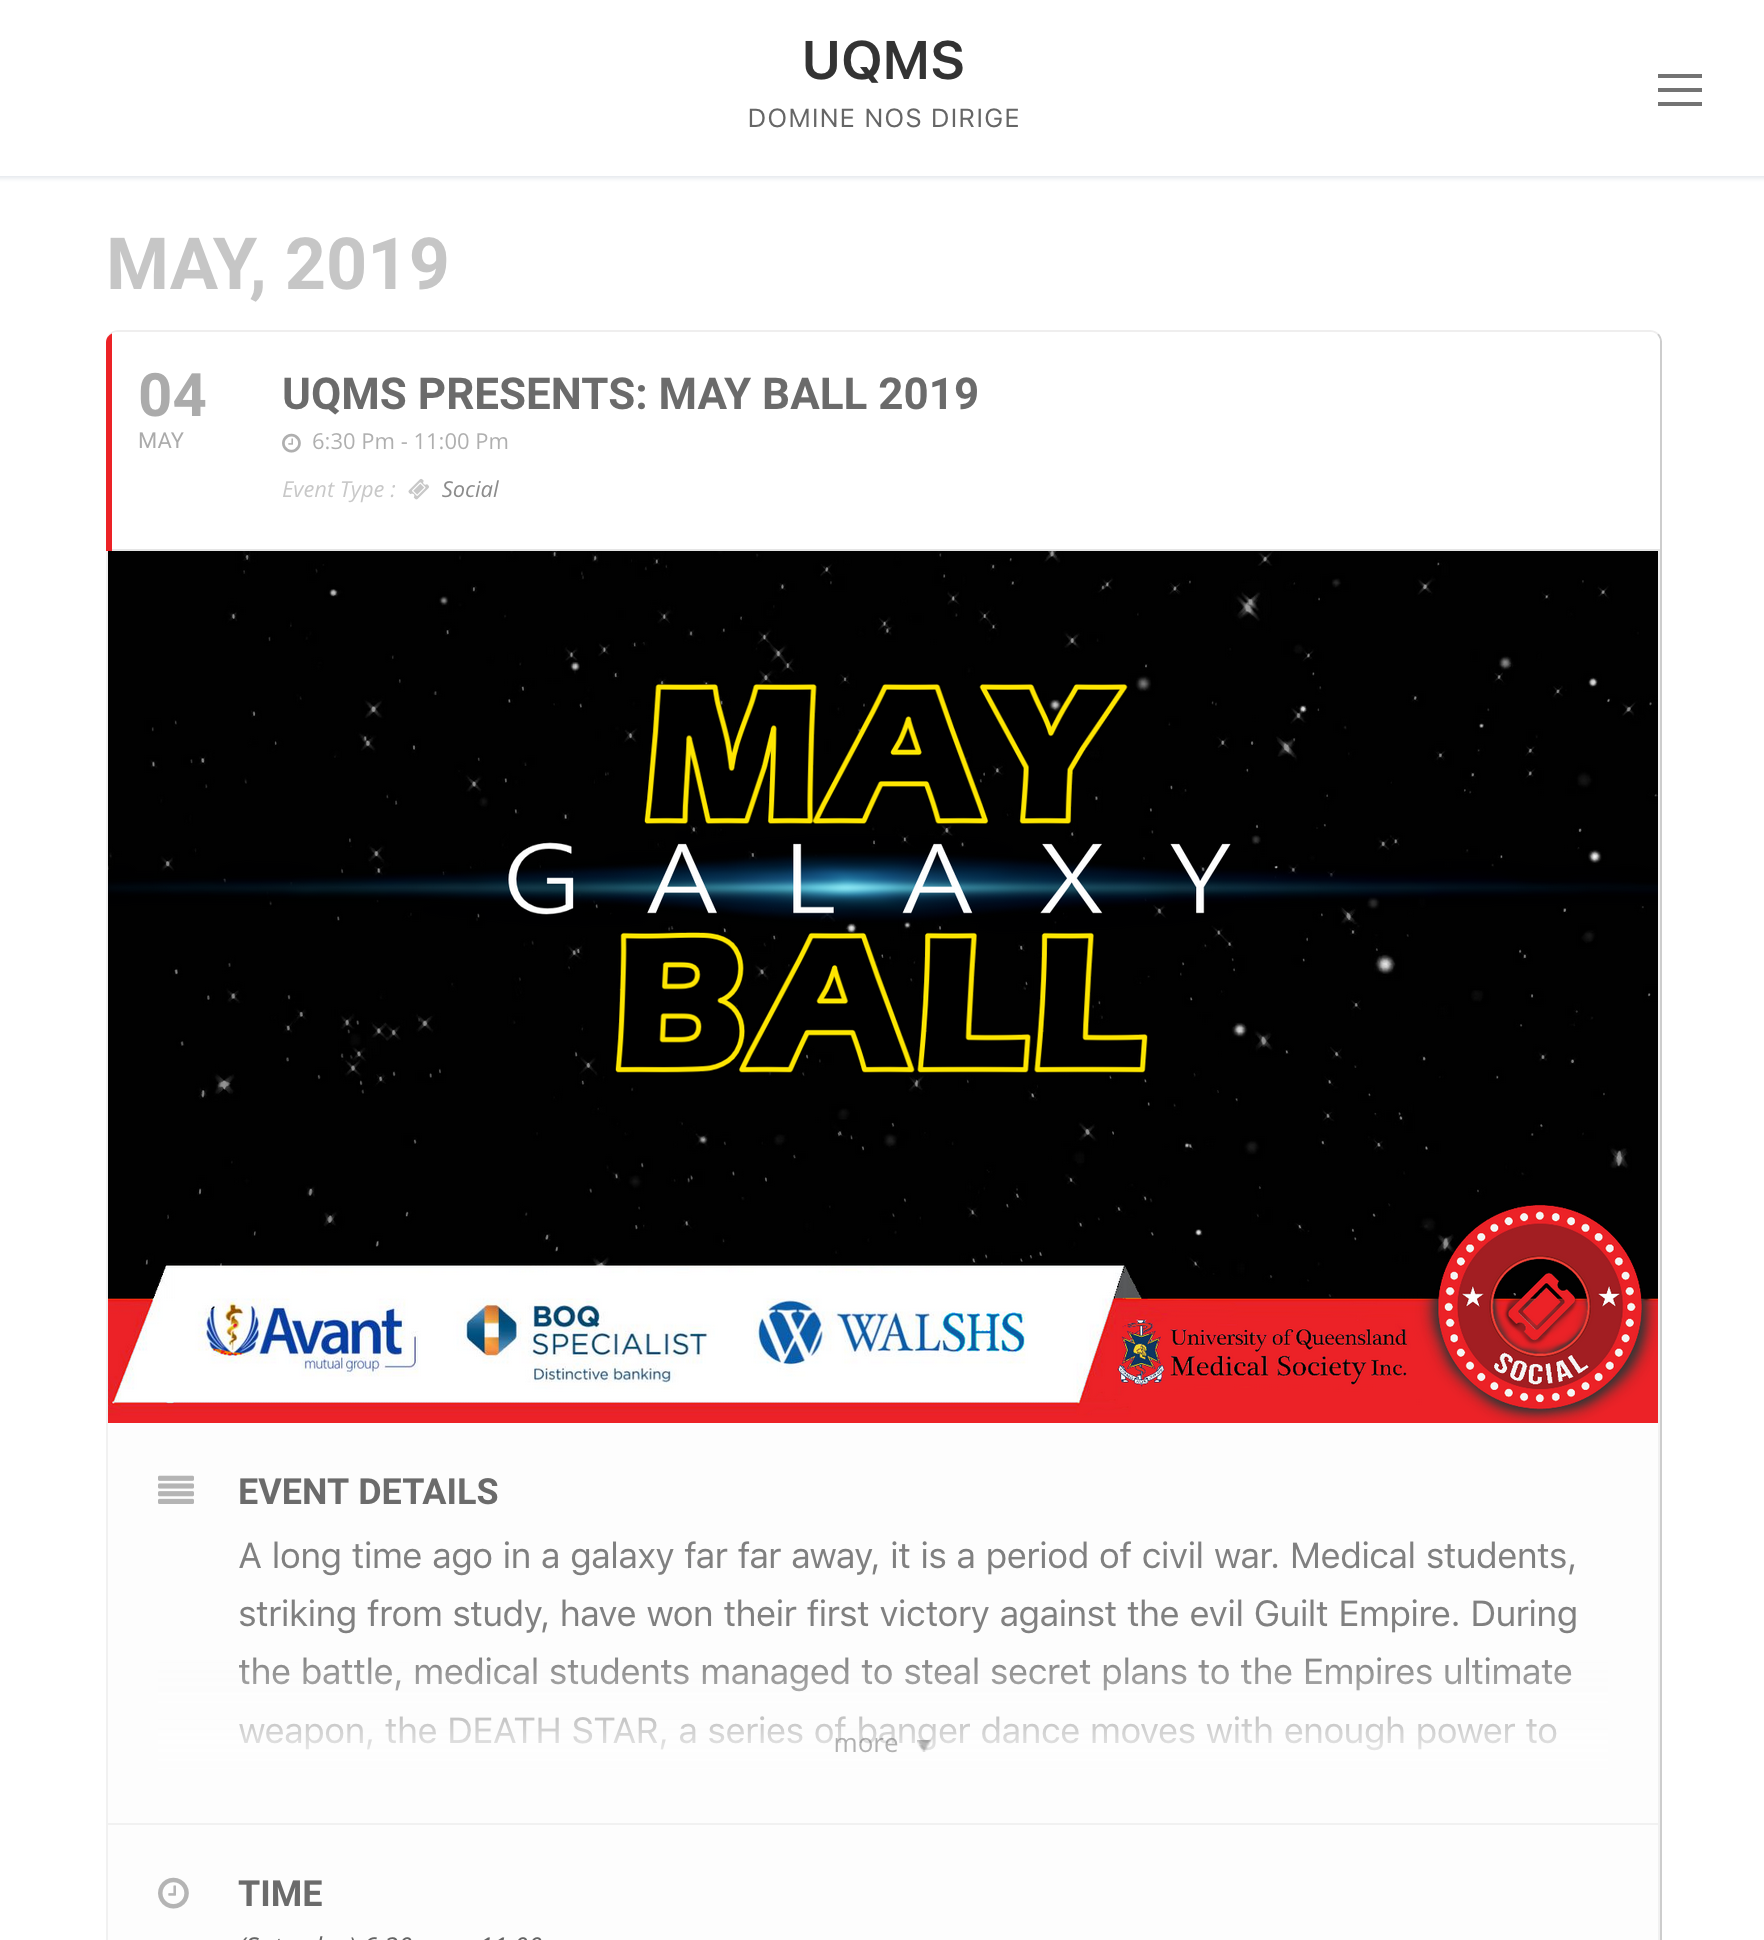
\includegraphics[width=0.7\linewidth]{mayball}
	\caption{Screenshot of the event page for the 2019 May Ball hosted by \gls{uqms}}\label{fig:uqms}
\end{figure}
All website should be accessible to their users and have support for people with impairments or a disadvantage. The \gls{wcag} outlines four key areas all websites should be assessed on and how these areas impact people and their use of the site. Figure~\ref{fig:uqms} shows a screenshot of the event page for the \gls{uqms} Ball in 2019, the accessibility of this site is as follows:
\begin{description}
	\item[Perceivable:] While all content is available upfront to the user, not all of the non-text content of the website has a text alternative. A lot of the images have not provided an \texttt{alt} attribute. However all of the content is presented visually in a simple one dimensional structure format, the choice in colours between the foreground and the background has resulted in a difficulty to view and read the content.
	\item[Operable:] The website is not operable purely from a keyboard, being able to view and read all of the content on the website requires the use of a mouse to expand the details. The navigation works as expected, allowing users to clearly and quickly identify where they are and being able to navigate to different pages easily through the menu.
	\item[Understandable:] The content is clearly sectioned and defined making it easy to read and understand what is being delivered. It follows a structure similar to other events pages and is clearly family upon opening.
	\item[Robust:] Upon inspecting the source of the website it is clear that the robustness of the website is lacking behind common web standards. An example is the clutter of div tags. With the lack of use of normal semantic \gls{html} tags and nesting content inside of \texttt{p} tags.
\end{description}


\subsubsection{Graceful Degradation}
\begin{figure}
	\centering
	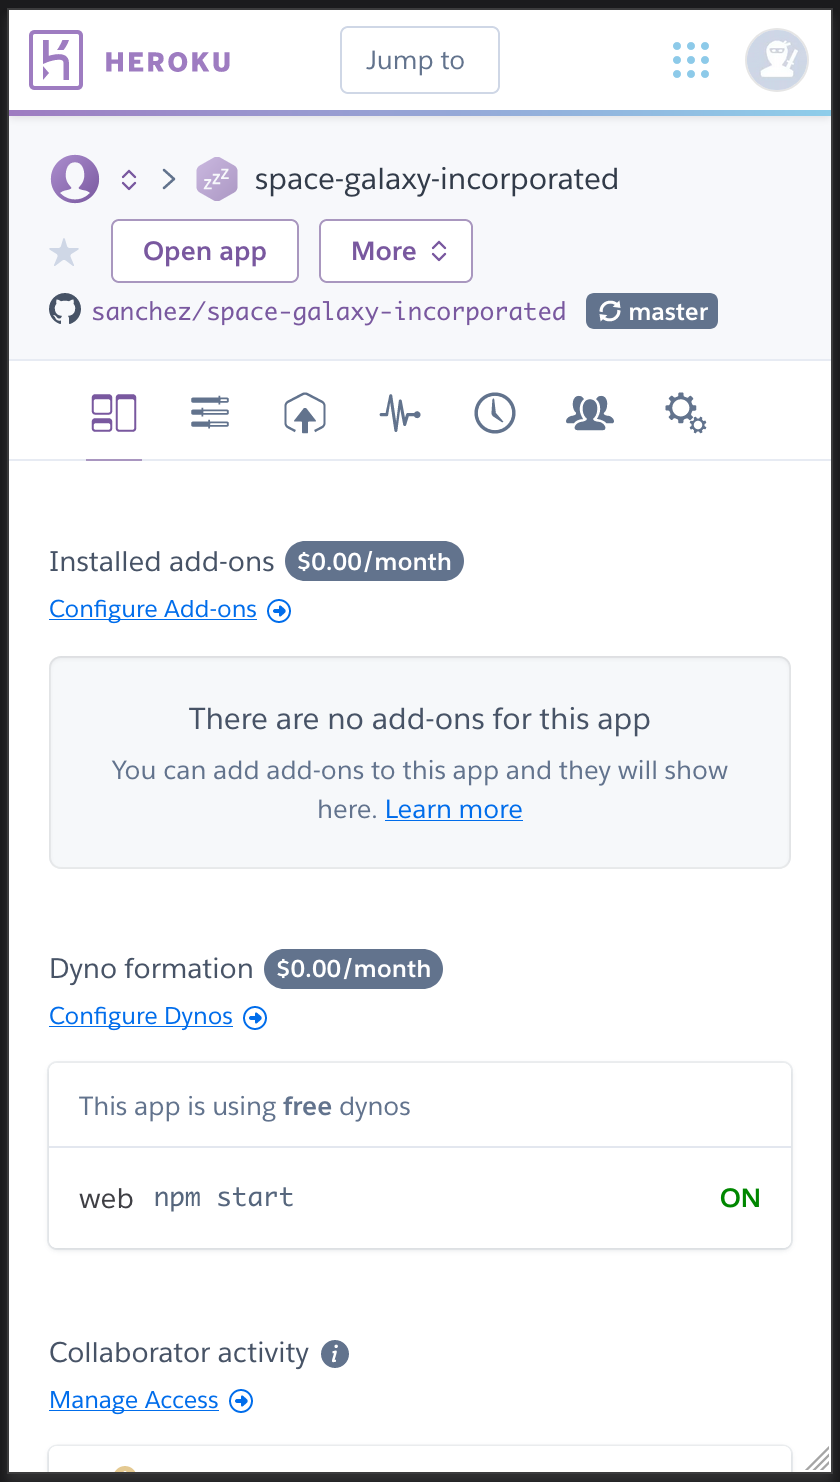
\includegraphics[width=0.3\linewidth]{heroku1}	
	\caption{Screenshot of the \gls{heroku} dashboard in a mobile view}\label{fig:heroku}
\end{figure}

An example of graceful degradation is the \gls{heroku} administrator dashboard. Figure~\ref{fig:heroku} shows the site in a mobile view, graceful degradation is applied here because the site is still usable, however some of the float controls have been wrapped around and not displayed as mobile friendly as possible. The ``Open App'' button could be collapsed into the ``More'' button and relabelled to represent a hamburger icon. The website overall is useful as a mobile application however, therefore the site gracefully degrades from desktop to mobile.

\subsubsection{Progressive Enhancement}
\begin{figure}
	\centering
	\subfloat[Mobile version of \gls{bootstrap}'s checkout]{
		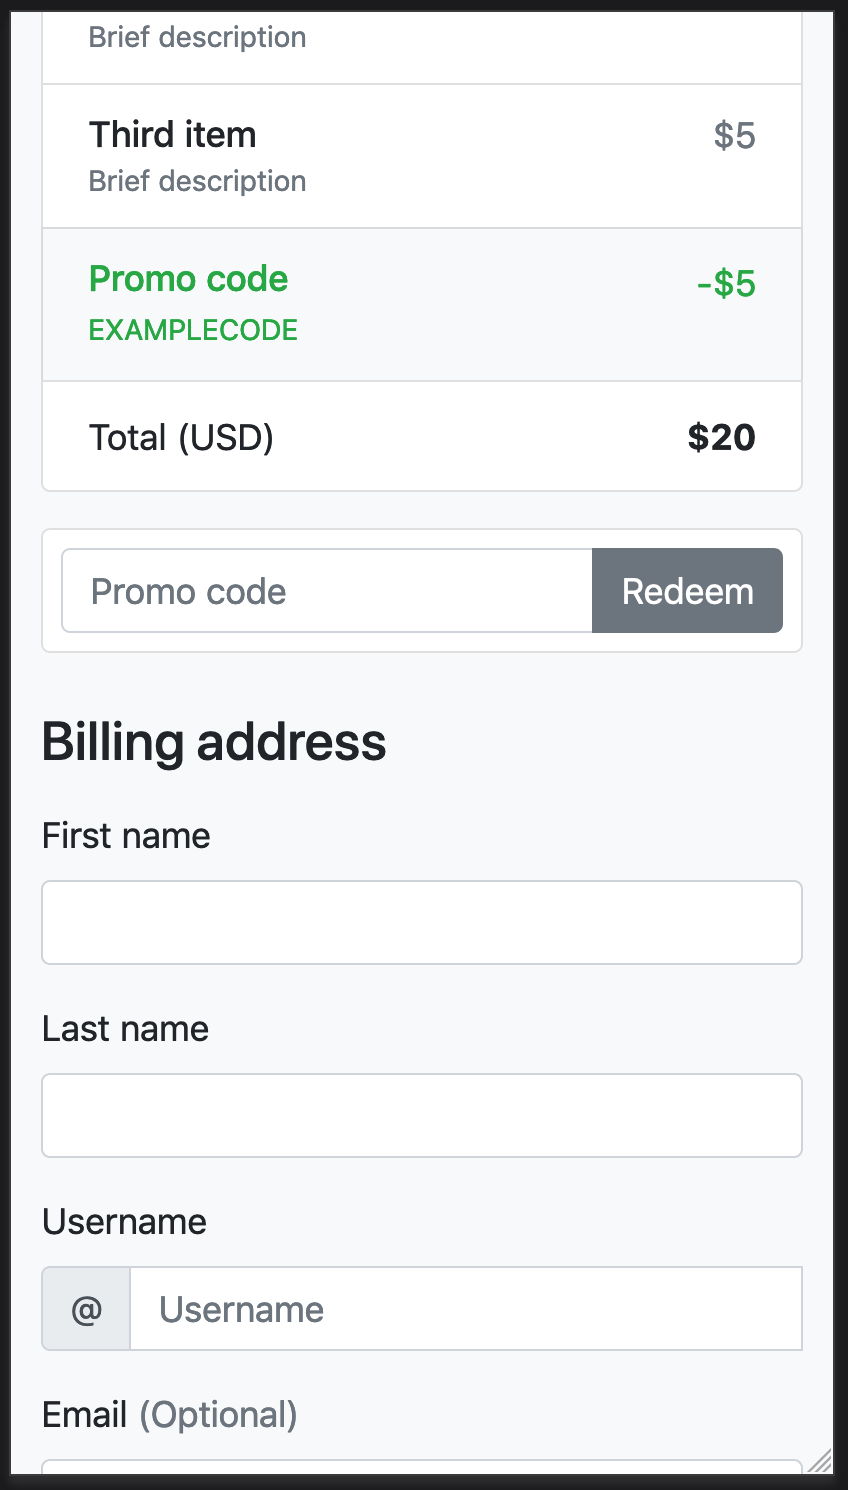
\includegraphics[width=0.3\textwidth]{bootstrap2}\label{fig:bootstrap:mobile}}
	\qquad
	\subfloat[Desktop version of \gls{bootstrap}'s checkout]{
		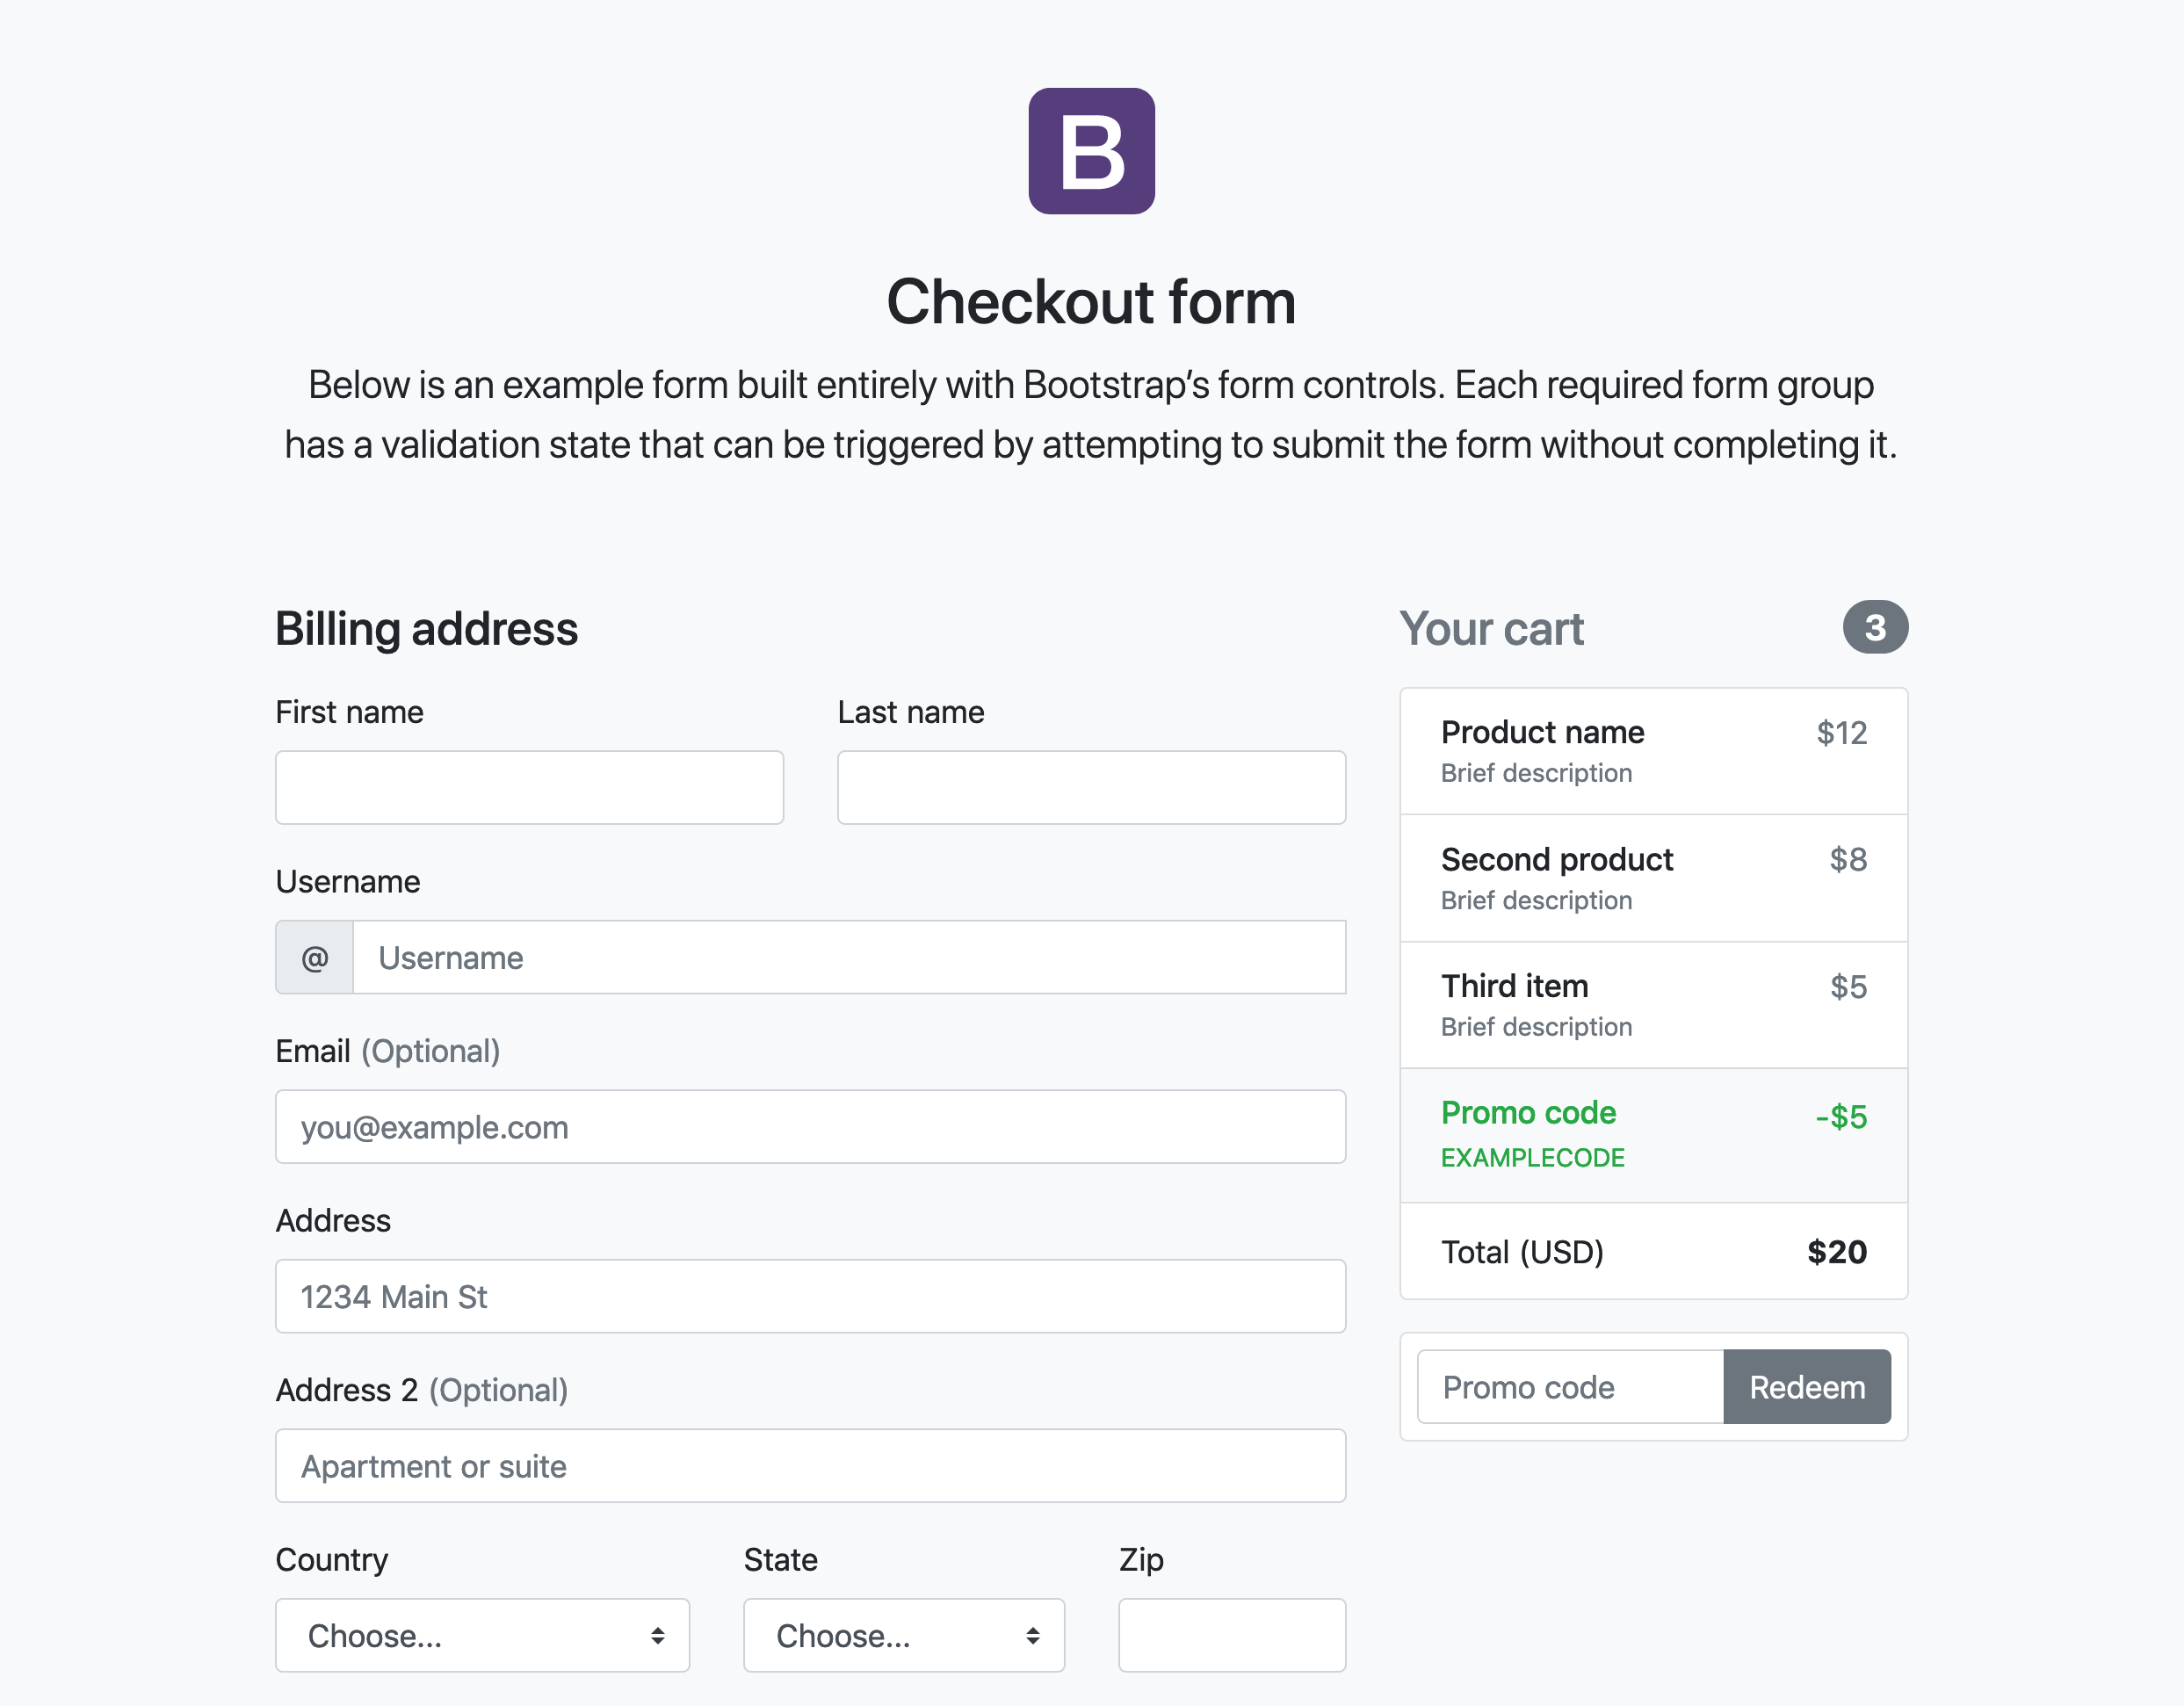
\includegraphics[width=0.6\textwidth]{bootstrap3}\label{fig:bootstrap:desktop}}
	\caption{Screenshots of \gls{bootstrap}'s example checkout page}\label{fig:bootstrap}
\end{figure}

\gls{bootstrap} is a perfect example of progressive enhancement, because the entire framework is around mobile-first design. Mobile-first design forces the designer to design the website with mobile in mind first and then once the site is designed mobile it can be scaled up to desktop with extra features being added and removed based on the screen size. Figure~\ref{fig:bootstrap} shows a comparison of the website between the mobile and desktop.\\\\
As seen in Figure~\ref{fig:bootstrap:mobile} the checkout list appears in the list however in Figure~\ref{fig:bootstrap:mobile} the list appears on the right side of the page. This design choice means the user is presented with the most important content first in mobile view but following common checkout design patterns in desktop view. This is achieved using media queries with respect to the window size, allowing for the window to be flexible and the mobile page is presented if the desktop screen size is too small.\\\\
Another notable difference is in the layout of the form for the billing address. In the desktop there are multiple columns of fields, but on the mobile version everything is one dimensional (all the fields flow down the page). This is achieved using both flexboxes to define the way content should flow in the page, and media queries to define the size of the columns and content inside the columns.

\subsubsection{Reflection}
It is clear that a direction of either degradation or enhancement is needed to be chosen. Since the website is primarily focussed at users on a computer (since \gls{git} is desktop only tool), the main focus will be on desktop devices and the website will gracefully degrade to support mobile devices. The accessibility of the website can be reinforced by picking more contrasting colours to help with identification of sections, and the use of more semantic \gls{html} can help improve the robustness.

\subsection{Security \& Privacy}
% What were the key things you learned from your Security \& Privacy group discussions?
% Write brief responses of your own to the guiding questions for these group discussions
\subsubsection{Security}
\begin{figure}
	\centering
	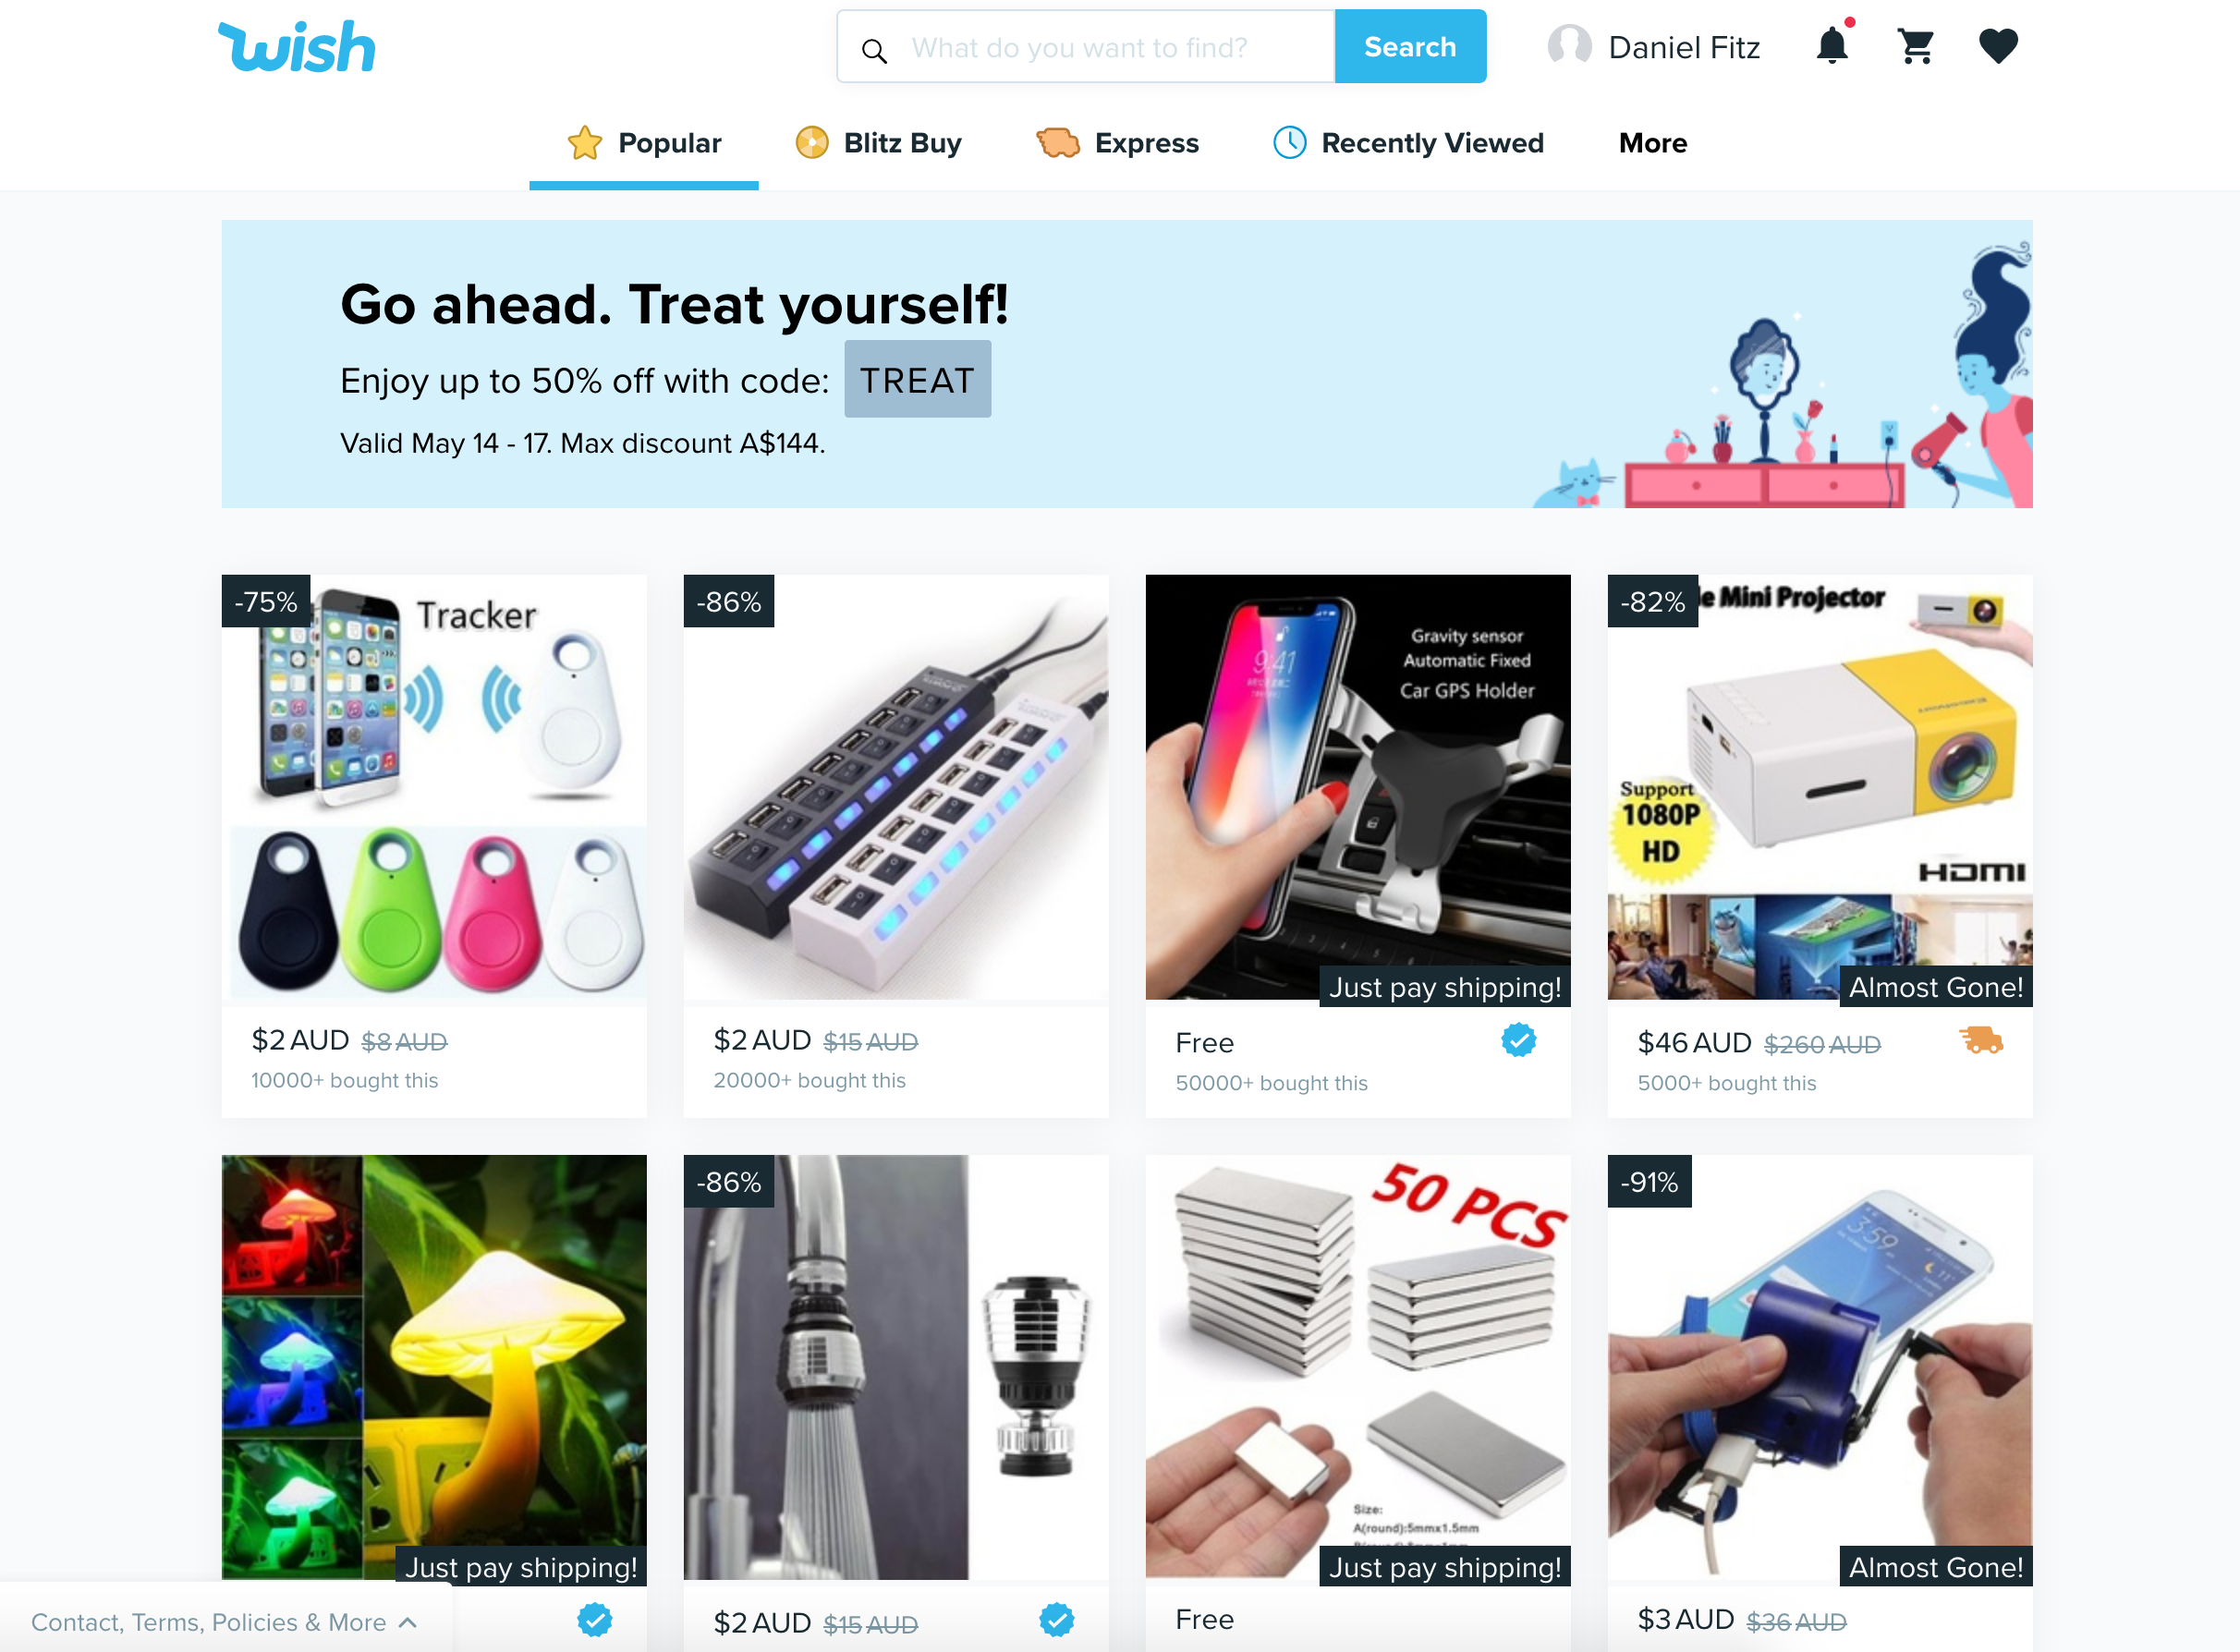
\includegraphics[width=0.8\linewidth]{wish}
	\caption{Screenshot of the homepage of a Wish.com site}\label{fig:wish}
\end{figure}
Security plays a massive role in modern web consumption, especially with ecommerce sites such as Wish.com. Wish.com is a site for buying and selling items online at really cheap prices. Figure~\ref{fig:wish} shows a screenshot of the landing page of Wish.com, some initial security threats are alerted when evaluating this website:
\begin{itemize}
	\item A lot of the items are so cheap it can sort of feel like a quick and dirty scam
	\item There is little to no descriptions about the items for sale
	\item The images of the items do not look representative of the real items
	\item The site attempted to run Flash scripts
	\subitem Flash has long been considered a threat to web security due to the access it has to the underlying \gls{os}	
\end{itemize}
While these are some strong security threats, Wish.com also has some good security initiatives in place to protect itself and the users:
\begin{itemize}
	\item The website is clean and unclustered
	\item There is a review system and a seller review system
	\item Purchases can be made using \gls{paypal}
	\item The site forces the use of \gls{https}
	\subitem The certificate is however verified and assigned to GoDaddy, which a relationship is not mentioned on the site anywhere	
\end{itemize}

\subsubsection{Privacy}
\begin{figure}[H]
	\centering
	
\includegraphics[width=0.7\linewidth]{betoota}
	\caption{Screenshot of a news article on The Betoota Advocate}\label{fig:betoota}
\end{figure}
User privacy is important to not only be aware of but to also respect too. The Betoota Advocate is a popular website providing news articles to users, news article providers benefit greatly from trackers and advertisements. However Betoota is different because Ghostery has alerted that there are no advertisements and only three trackers used in the article being observed (Figure~\ref{fig:betoota}). On top of the minimal trackers and advertisements, Betoota also has minimal cookies in use (10 cookies in total) most of which are related to third-party tools or services the site uses.

\subsection{Hi-Fi User Testing}
% Reflect on the success of the Hi-Fi User Testing design activity you did in Week 13
% Include the testing plan you developed for the activity
% Include photos you took of the activity running
% What feedback did you get and how did it inform your final product?
For the Hi-Fi User Testing task there were five main instructions requested from the user to complete during the session:
\begin{enumerate}
	\item Learn the basics of Git
	\subitem Observe the speed at which the user consumes the knowledge on the homepage
	\item Access the Quizzes page
	\subitem Observe if they look for a link on the homepage or in the navigation bar
	\item Find an advanced command
	\subitem Observe if they scroll through the page and look for an advanced looking command or jump to the references page
	\item Complete the first question involving the terminal sandbox
	\subitem Observe how the user interacts with the sandbox, is there clear direction to their actions
	\item Create a branch in the terminal sandbox
	\subitem Observe if the user switches back to the main tutorial to look for commands
\end{enumerate}
Upon initial observations it became clear that users were unable to realise the site could be scrolled and the homepage contained content past the first screen. This set back placed a lot of users in a place of confusion and frustration already. Therefore when they realised they could scroll they really quickly skimmed through all the content without properly observing the information and reading.\\\\
Access the quizzes page was done primarily through the use of the navigation bar, with only one user looking at the bottom of the page for a quiz link after reading the content.\\\\
The advanced command however, most users thought an advanced command was a command covered on the page and had no idea there were more commands hidden in the references page.\\\\
Both tasks involving the the \gls{git} sandbox resulted in the users not being able to understand how to use the sandbox and not knowing what commands to use. Some of the users also noted they had no idea the text in the grey boxes were commands that could be run in the sandbox.

\subsubsection{Reflection}
Upon receiving this feedback it was clear some adjustments were required to get the product up a standard that is usable for users. Some minor changes are needed to be made to fix the issues people had with the Hi-Fi test:
\begin{itemize}
	\item Add an arrow or some indication on the first screen to inform users that they can scroll down. Also make this action interactive so that if the user clicks on it they will be moved down to the next section.
	\item Make the side menu more noticeable via the use of some animation, most users were not aware it could be used or even existed.
	\item Add a final paragraph that links to the other pages as an indicator for the next steps the user can take.
	\item Add some tooltips to both the command boxes and the \gls{git} sandbox to help the user understand what the content is for and how to use it.
\end{itemize}






	
	% !TeX spellcheck = en_US
% !TeX root = main.tex

\chapter{Conclusion}
% Summarise and conclude your Design Report
% In short, how has your website been successful in responding to the brief?

\section{Course Reflection}
% How has your learning strategy changed since the start of the course?
% If you had the change to restart, how would you approach your learning differently?
	
	\newpage
	\addcontentsline{toc}{chapter}{References}
	\bibliographystyle{ieeetr}
	\bibliography{bib}
	
\end{document}